
\section{Experimentación}
En esta sección experimentaremos variando la dificultad del Proof-Of-Work y la cantidad de nodos, y mediremos el tiempo de ejecución. Para correr la experimentación se utilizó una computadora con un procesador \textit{Intel(R) Core(TM) i7-8550U CPU @ 1.80GHz} con cuatro cores.

\begin{figure}[H]
	\centering
	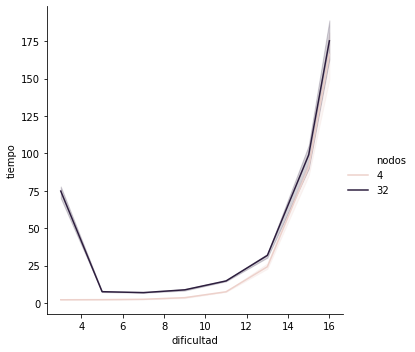
\includegraphics[width=0.7\linewidth]{img/grafico}
	\caption{Tiempo en función de dificultad para distinta cantidad de nodos.}
	\label{fig:grafico}
\end{figure}

En la Figura \ref{fig:grafico} podemos ver que cuando hay pocos nodos, el tiempo de ejecución crece muy rápidamente al subir la dificultad. En cambio, cuando hay muchos nodos, con dificultades muy chicas el tiempo es mayor y a medida que la dificultad aumenta, este disminuye hasta un punto en el que vuelve a aumentar.

Este comportamiento coincide con lo esperado a partir de nuestro análisis del protocolo. Cuando hay pocos nodos, 
la carga sobre la red es pequeña, sin importar la dificultad,
la cual varía que tan rápido se generan nuevos bloques. Luego el tiempo de generación de bloques se vuelve 
predominante sobre el tiempo de sincronización.

Cuando hay muchos nodos y la dificultad es baja,
es mayor el tiempo que se necesita para sincronizar las cadenas, a la vez que muchos bloques son 
desperdiciados. Al aumentar la dificultad, la cantidad de mensajes se reduce, y el tiempo necesario
para la sincronización también, luego el tiempo de producción de bloques se vuelve nuevamente predominante.
Es por esta razón, que vemos al tiempo de ejecuci\'on primero disminuir y luego volver a aumentar. A largo plazo, dado que la dificultad crece de forma exponencial, el tiempo de sincronizaci\'on se vuelve despreciable y es por esto que ambas curvas convergen.